\documentclass{article}
\usepackage[margin=1in]{geometry}
\usepackage{amsmath,amsthm,amssymb}
\usepackage{bbm,enumerate,mathtools}
\usepackage{tikz,pgfplots}
\usepackage{chessboard}
\usepackage[hidelinks]{hyperref}
\usepackage{multicol} % Problem 35

\newenvironment{question}{\begin{trivlist}\item[\textbf{Question.}]}{\end{trivlist}}
\newenvironment{note}{\begin{trivlist}\item[\textbf{Note.}]}{\end{trivlist}}
\newenvironment{references}{\begin{trivlist}\item[\textbf{References.}]}{\end{trivlist}}
\newenvironment{related}{\begin{trivlist}\item[\textbf{Related.}]\end{trivlist}\begin{enumerate}}{\end{enumerate}}


\begin{document}

\rating{1}{2}
Given some set of functions $\{p_i \colon [n] \rightarrow [k]\}_{i=1}^m$
consider the semigroup generated by $\langle p_1, p_2, \dots, p_m\rangle$.

\begin{figure}[ht!]
  \center
  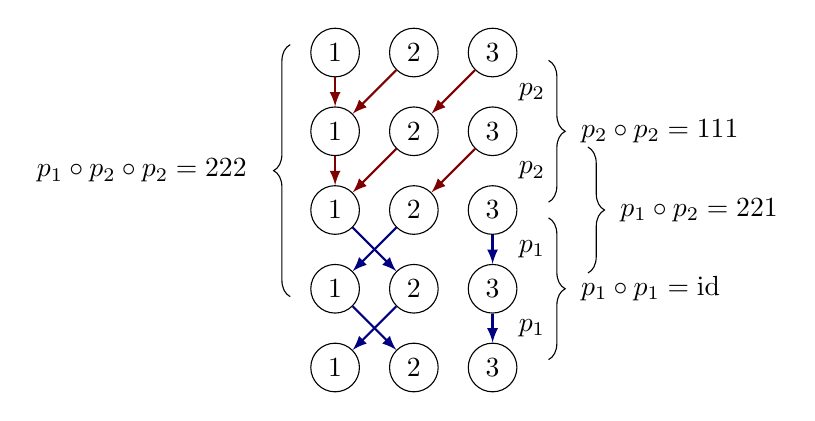
\begin{tikzpicture}
    \foreach \x in {1,2,3} {
      \foreach \y in {1,2,3,4,5} {
        \node[draw, circle] (\x\y) at (\x,\y) {\x};
      }
    }
    \path[->, thick, >=latex, red!50!black]
      (15) edge (14) (25) edge (14) (35) edge (24)
      (14) edge (13) (24) edge (13) (34) edge (23)
    ;
    \path[->, thick, >=latex, blue!50!black]
      (13) edge (22) (23) edge (12) (33) edge (32)
      (12) edge (21) (22) edge (11) (32) edge (31)
    ;
    \node (p11) at (3.5, 1.5) {$p_1$};
    \node (p12) at (3.5, 2.5) {$p_1$};
    \node (p21) at (3.5, 3.5) {$p_2$};
    \node (p22) at (3.5, 4.5) {$p_2$};
    \draw [decorate,decoration={brace, amplitude=6pt},xshift=6pt] (3.5,2.9) -- (3.5,1.1);
    \node[anchor=west] at (4,2) {$p_1 \circ p_1 = \mathrm{id}$};
    \draw [decorate,decoration={brace, amplitude=6pt},xshift=6pt] (3.5,4.9) -- (3.5,3.1);
    \node[anchor=west] at (4,4) {$p_2 \circ p_2 = 111$};
    \draw [decorate,decoration={brace, amplitude=6pt},xshift=6pt] (4,3.8) -- (4,2.2);
    \node[anchor=west] at (4.5,3) {$p_1 \circ p_2 = 221$};
    \draw [decorate,decoration={brace, amplitude=6pt},xshift=-2pt] (0.5,1.9) -- (0.5,5.1);
    \node[anchor=east] at (0,3.5) {$p_1 \circ p_2 \circ p_2 = 222$};
  \end{tikzpicture}
  \caption{Given $p_1 = 213$ and $p_2 = 112$, there are six distinct functions that
  can be made from nonempty compositions of these functions: $p_1$, $p_1 \circ p_1$, $p_1 \circ p_2$, $p_1 \circ p_2 \circ p_2$, $p_2$, and $p_2 \circ p_2$.}
\end{figure}

\begin{question}
  If the $p_i$s are chosen uniformly at random, what is the expected size of the
  semigroup?
\end{question}

\begin{related}
  \item What's the expected number of functions $m$ such that
    $|\langle p_1, p_2, \dots, p_m\rangle| = k^n$? The minimum number of
    functions?
  \item What is the largest semigroup as a function of $n$, $k$, and $m$?
  \item Can you make any size semigroup with the right parameters? If not,
    what sizes can you make?
\end{related}

\begin{references}
  \item Problem 6.
\end{references}
\end{document}
